\section{Control Plots}
%%%%%%%%%%%%%%%%%%%%%%%%%%%%%%%%%%%%%%%%%%%%%%%%%%%%%%%%%%%%%%%%%%%%%%
\label{sec:ControlPlots}

\subsection{Signal and background yields}\label{subsec:yields}
In table \ref{table:yields} are reported the expected number of events for signals and backgrounds after the full analysis selection. The uncertainties in the expected number of events correspond to the prefit nuisances effect affecting each process. As can be observed, signals are splitted into different categories depending on the production mode: gluon fusion (ggH), VBF (qqH) and VH (WH and ZH) which includes also ttH production. Each signal is again splitted in six different contributions related to the \pth bins. The total expected signal yield after the analysis selection is $382 \pm 7$ events.\\
For what the backgrounds are concerned, the WW has been splitted in bins of \pth and has been left free to float independently in each bin during the fit. For doing this a 100 \% uncertainty has been associated to the expected number of events in each bin, following a prior flat distribution (log uniform distribution). That is why the uncertainty on WW backgrounds and on total background yield are not reported in the table.\\
The Top background has been divided into two categories of events as explained in \ref{sec:TTBackground}: events with zero jets (Top0jet) and events with more than zero jets (Topge1jet). The yield in the first category has been extracted performing a data driven estimation in a control region. The latter category has been further splitted in the various \pth bins and a data driven estimation has been performed separately in each bin to avoid a shape mismodelling in the \pth distribution for this background.\\
The final signal to background ratio is around 3~\%, consistent with what illustrated in figure \ref{fig:cutflow}.

\begin{table}[htbp]
\begin{center}
 {
\small{
\setlength{\extrarowheight}{2pt}
  \caption{Signal prediction, background estimates and observed number of events in data are shown in each \pth{} bin for the signal after applying the analysis selection requirements. The total uncertainty on the number of events is reported. For signal processes, the yield related to the ggH are shown, separated with respect to the contribution of the other production mechanisms (XH=VBF+VH). The WW process includes both quark and gluon induced contribution, while the Top process takes into account both $\mathrm{t\bar t}$ and tW. }\label{table:yields}
\begin{tabular} {l c c c c c c}
  \hline \hline
$\mathbf{p}_{\rm \mathbf{T}}^{\rm \mathbf{H}} \left[\mathrm{\mathbf{GeV}}\right] $	&	\bf{0-15}	&	\bf{15-45}	&	\bf{45-85}	&	\bf{85-125}	&	\bf{125-165}	&	\bf{165-$\boldsymbol{\infty}$} \\ 	

\hline

ggH	&	$73\pm3$	&	$175\pm5$	&                $59\pm3$	&                $15\pm2$	&                $5.1\pm1.5$	&                $4.9\pm1.4$	\\
XH=VBF+VH	&	$4\pm2$ 	&	$15\pm4$ 	&		 $16\pm4$	&	         $8\pm2$ 	&		 $3.8\pm1.1$ 	&		 $3.0\pm0.8$    \\	
Out-of-fiducial & $9.2\pm0.5$   &       $19.9\pm0.7$    &      $11.4\pm0.6$    &    $4.4\pm0.3$   &     $1.6\pm0.2$   &   $2.4\pm0.2$ \\
Data 	&	2182	 	&         5305	 	&	         3042	 	& 	          1263	 	&	         431	 	& 	          343	 	\\
Total background &  	 $2124\pm128$	 &     $5170\pm321$	 &       $2947\pm293$	 &            $1266\pm175$	 &         $420\pm80$	 &              $336\pm74$	 \\

WW 	& 		$1616\pm107$	 &	 $3172\pm249$	 &	     $865\pm217$	 &	     $421\pm120$	 &	     $125\pm60$	 &		     $161\pm54$	 \\
Top 	&	$184\pm38$	&	                $1199\pm165$	&	                $1741\pm192$	&	                $735\pm125$	&	                $243\pm51$	& 	        $139\pm49$	\\
W+jets 	& $134\pm5$ 	&	         $455\pm10$ 	&	         $174\pm6$ 	&	         $48\pm4$ 	&	         $14\pm3$ 	&	         $9\pm3$ 	\\
WZ+ZZ+VVV & $34\pm4$ 	 &	$107\pm10$ 	&                $71\pm7$ 	&	         $29\pm5$ 	&                $14\pm3$ 	&     $13\pm4$ 	\\
\dytt 	&	$23\pm3$ 	&         $67\pm5$ 	&         $47\pm4$ 	&         $22\pm3$ 	&         $12\pm2$ 	&         $10\pm2$ 	\\
W$\gamma^{(*)}$	& $132\pm49$     &             $170\pm58$    &              $48\pm30$ &                  $12\pm9$ &                  $3\pm3$ &                 $5\pm10$ \\
\hline

\hline
  \end{tabular}
  }
  }

  \end{center}
\end{table}

\subsection{Control plots in the signal region}
In figure \ref{fig:control_plots} are reported the control plots in the signal region for the \mll~ distribution in all the \pth bins. Data points are superimposed to MC distributions only in the high \mll~ region (above 70~\GeV), where no signal is expected. The error bands shown in these plots correspond to the total prefit uncertainty, taking into account all the sources of error. The very large uncertainties are expected and are related to the 100~\% uncertainty assigned to the WW floating background. The error band will decrease once the fit will be performed, i.e using the postfit values of the nuisance parameters, and the WW yield will be adapted to data.
\begin{figure}[htb]
\centering
\subfigure[Bin1]{
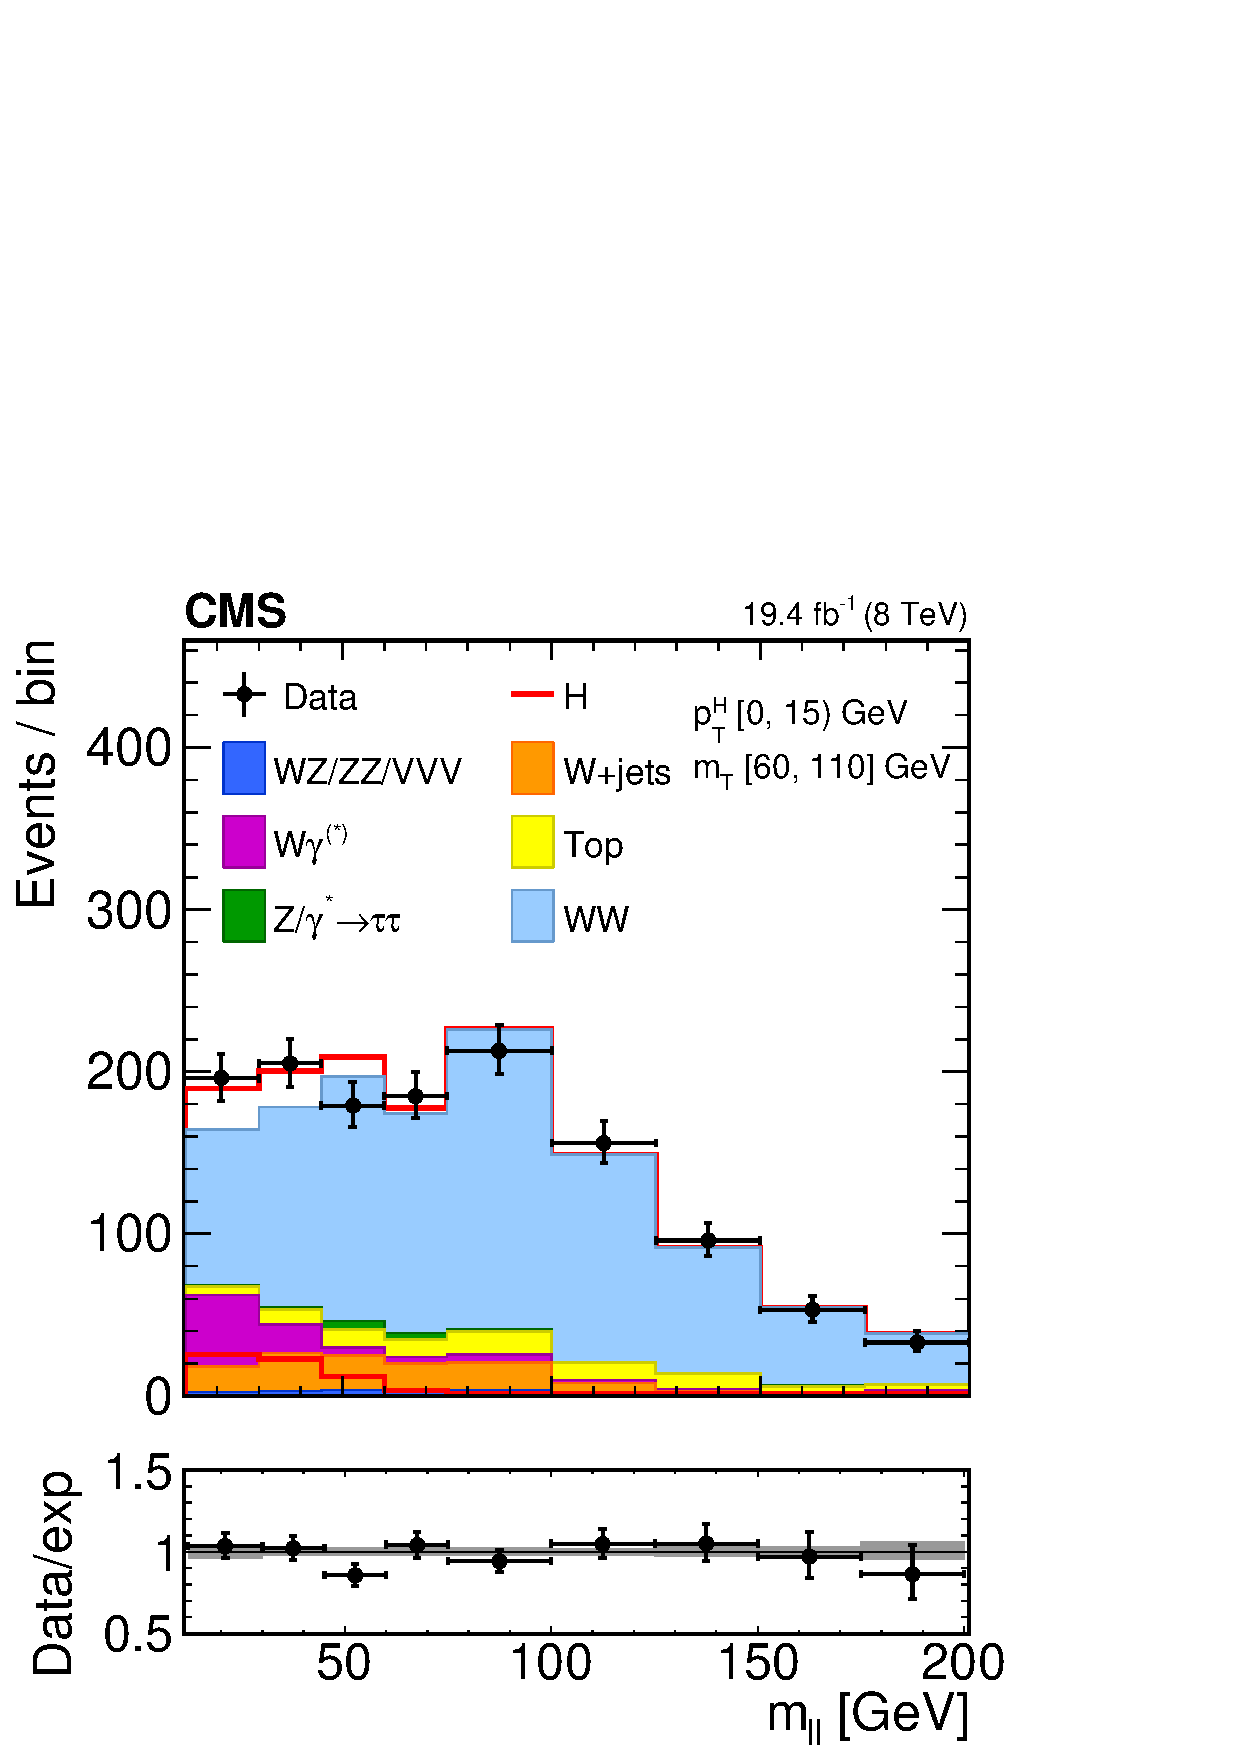
\includegraphics[width=0.35\textwidth]{images/mllBin0.pdf}
}
\subfigure[Bin2]{
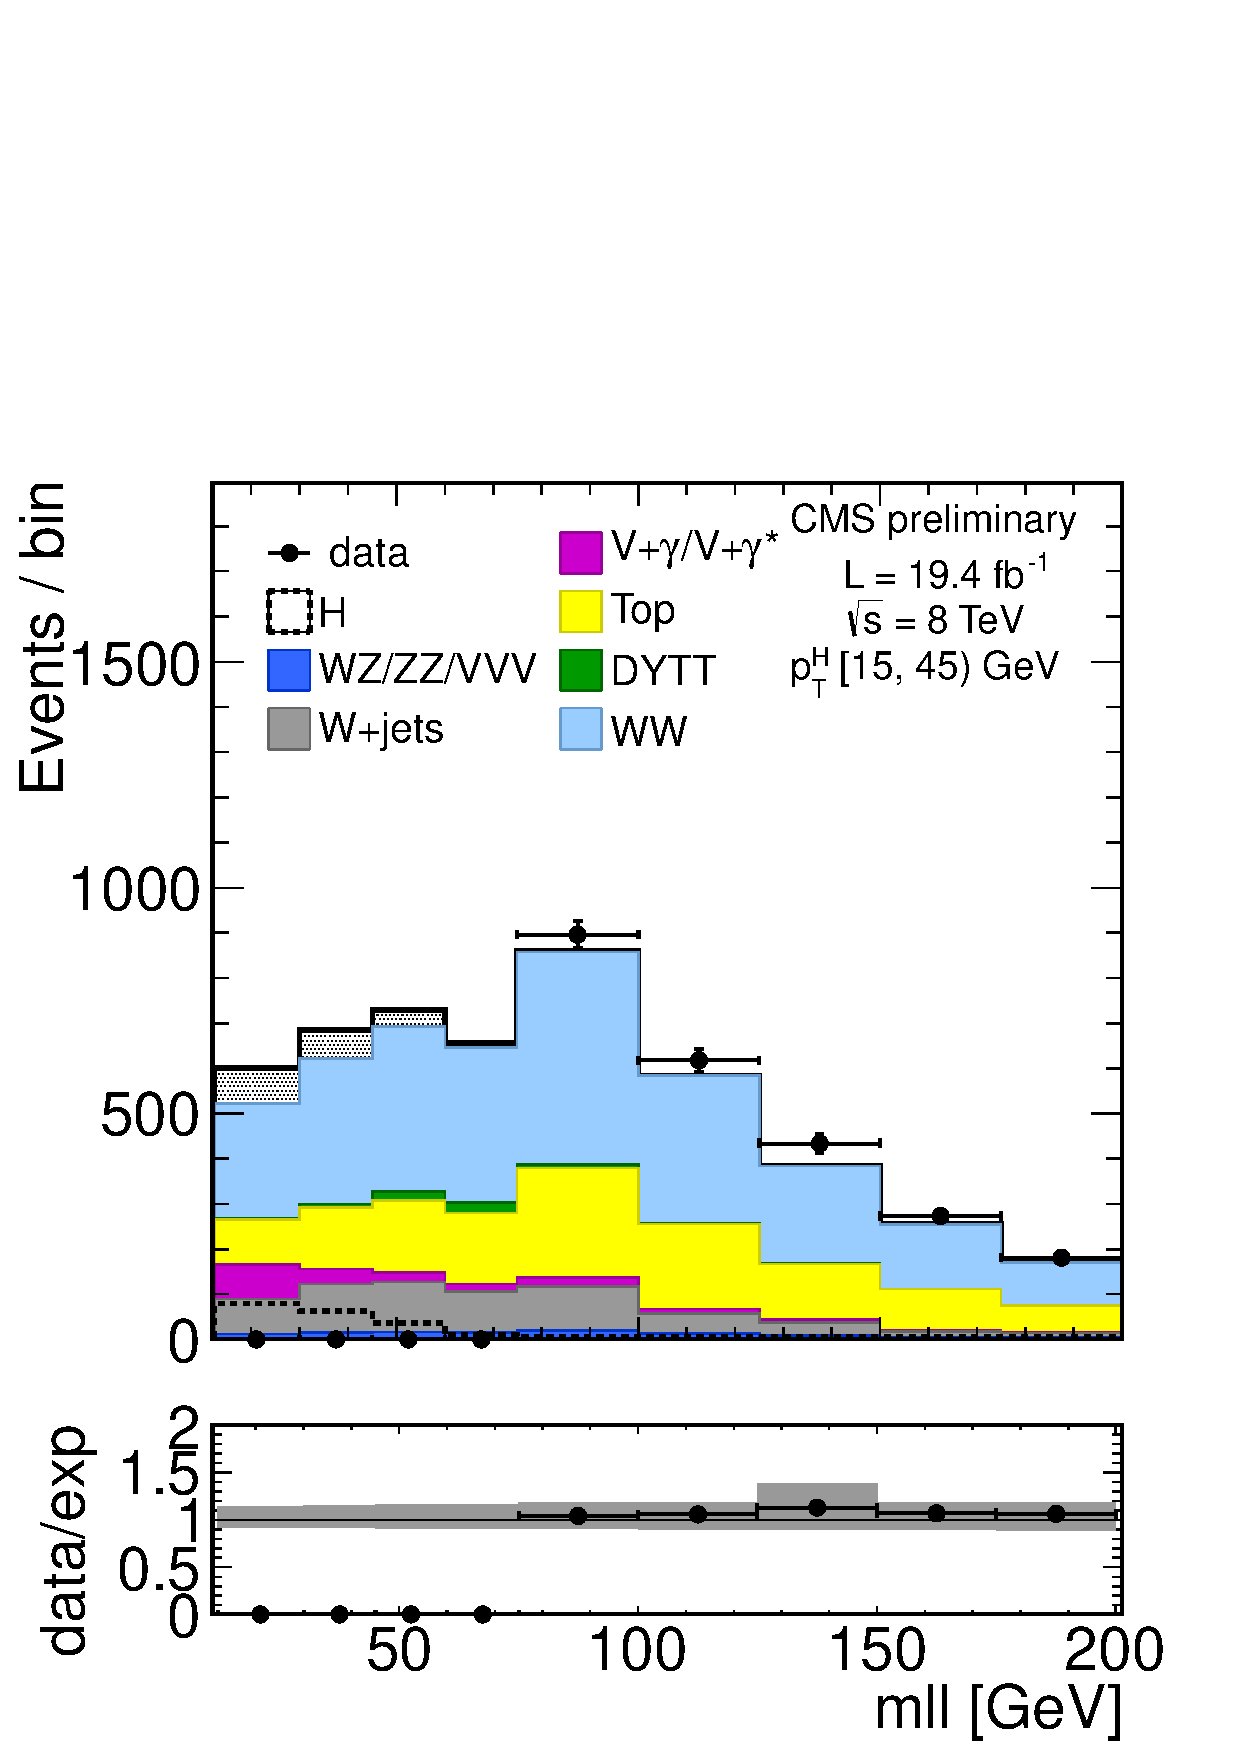
\includegraphics[width=0.35\textwidth]{images/mllBin1.pdf}
}
\\
\subfigure[Bin3]{
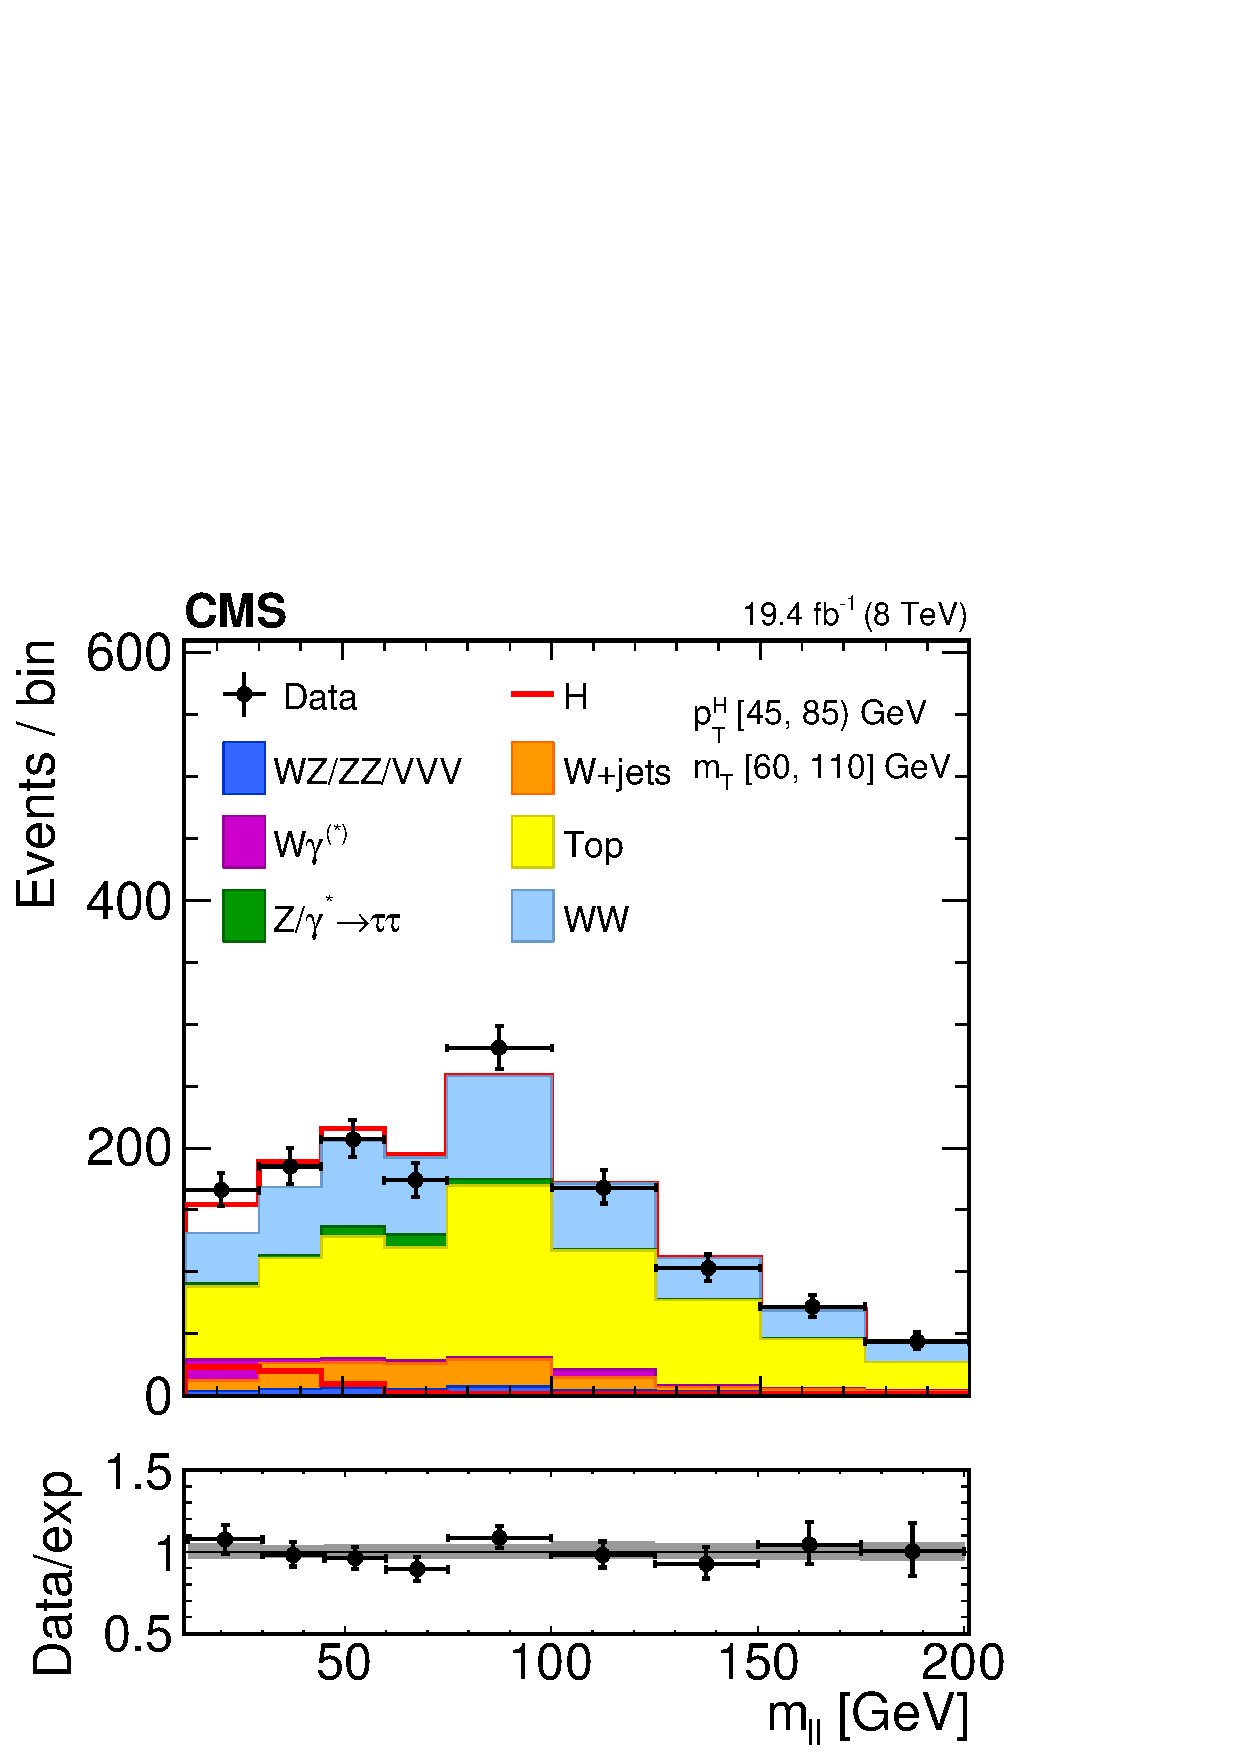
\includegraphics[width=0.35\textwidth]{images/mllBin2.pdf}
}
\subfigure[Bin4]{
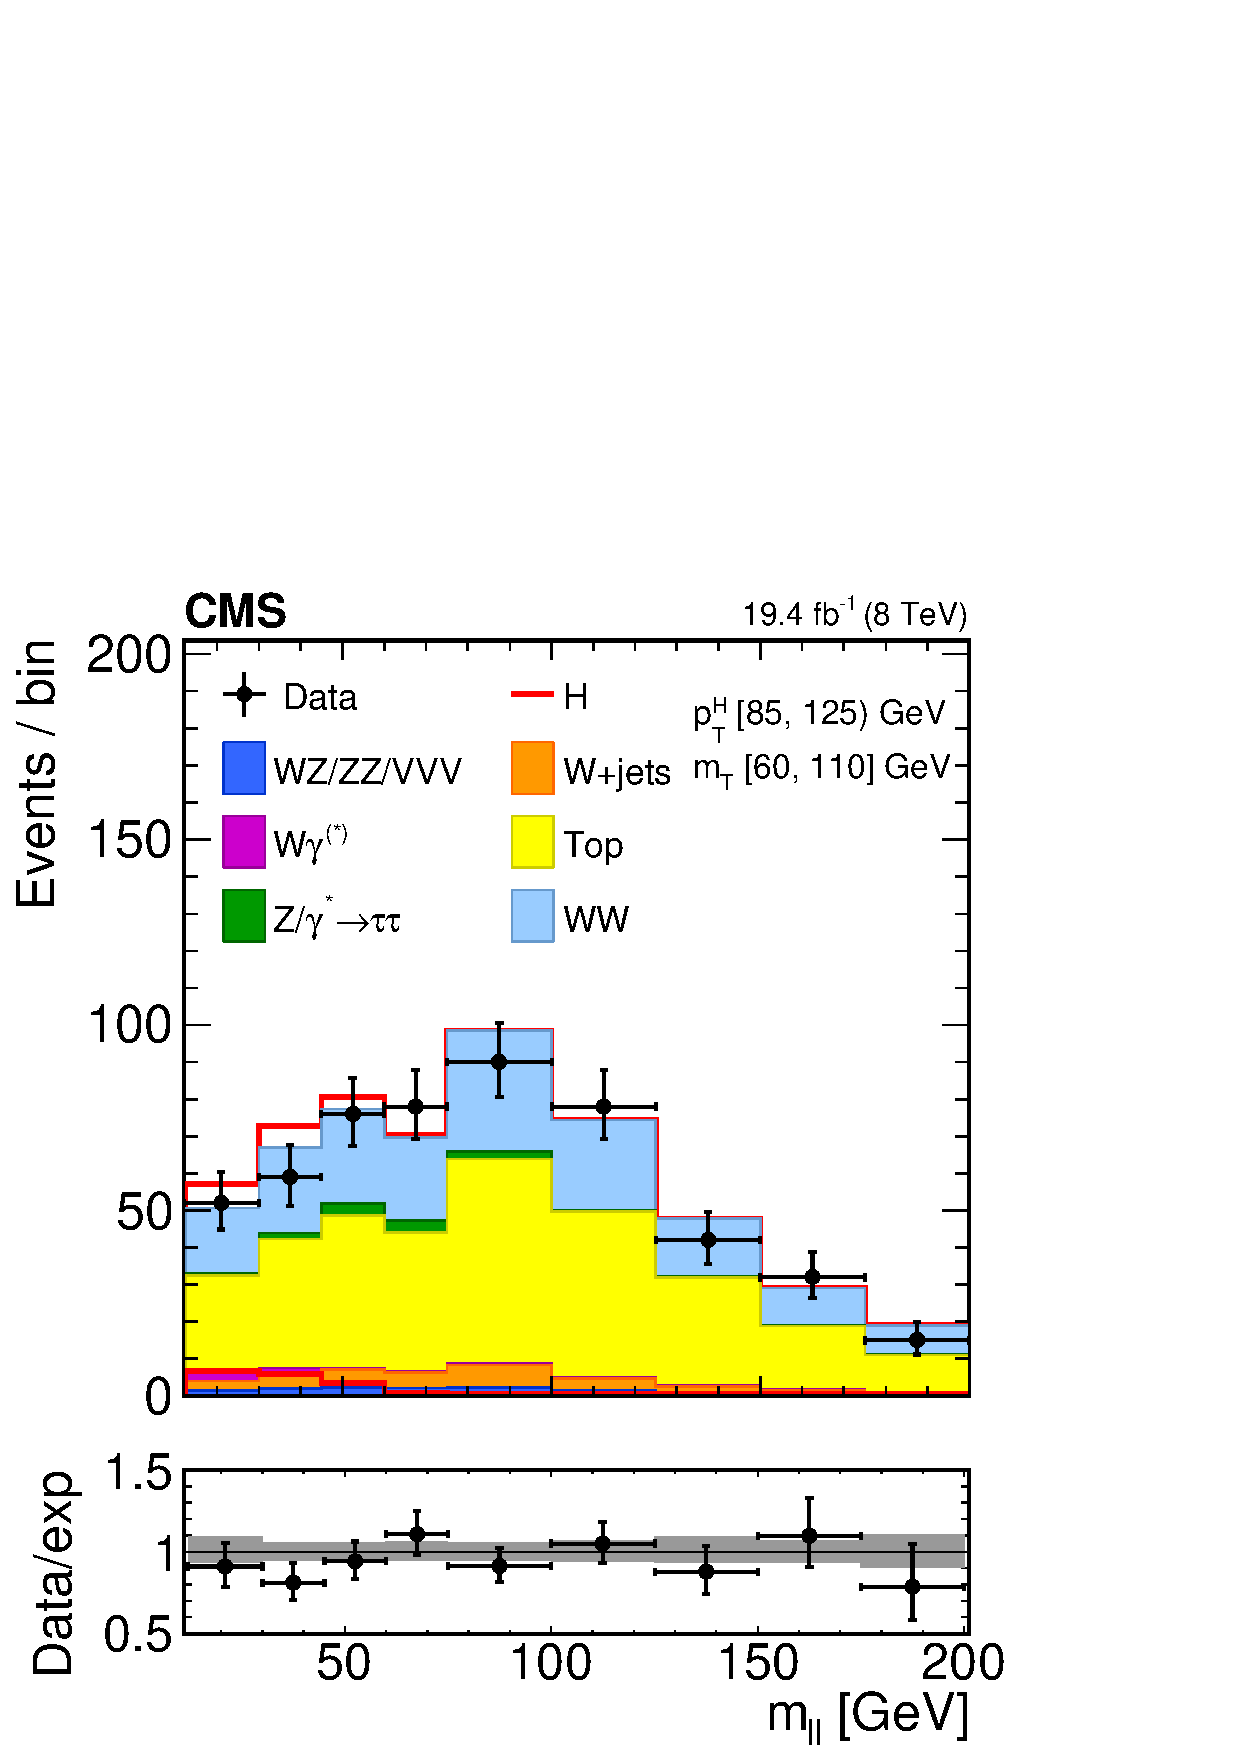
\includegraphics[width=0.35\textwidth]{images/mllBin3.pdf}
}
\\
\subfigure[Bin5]{
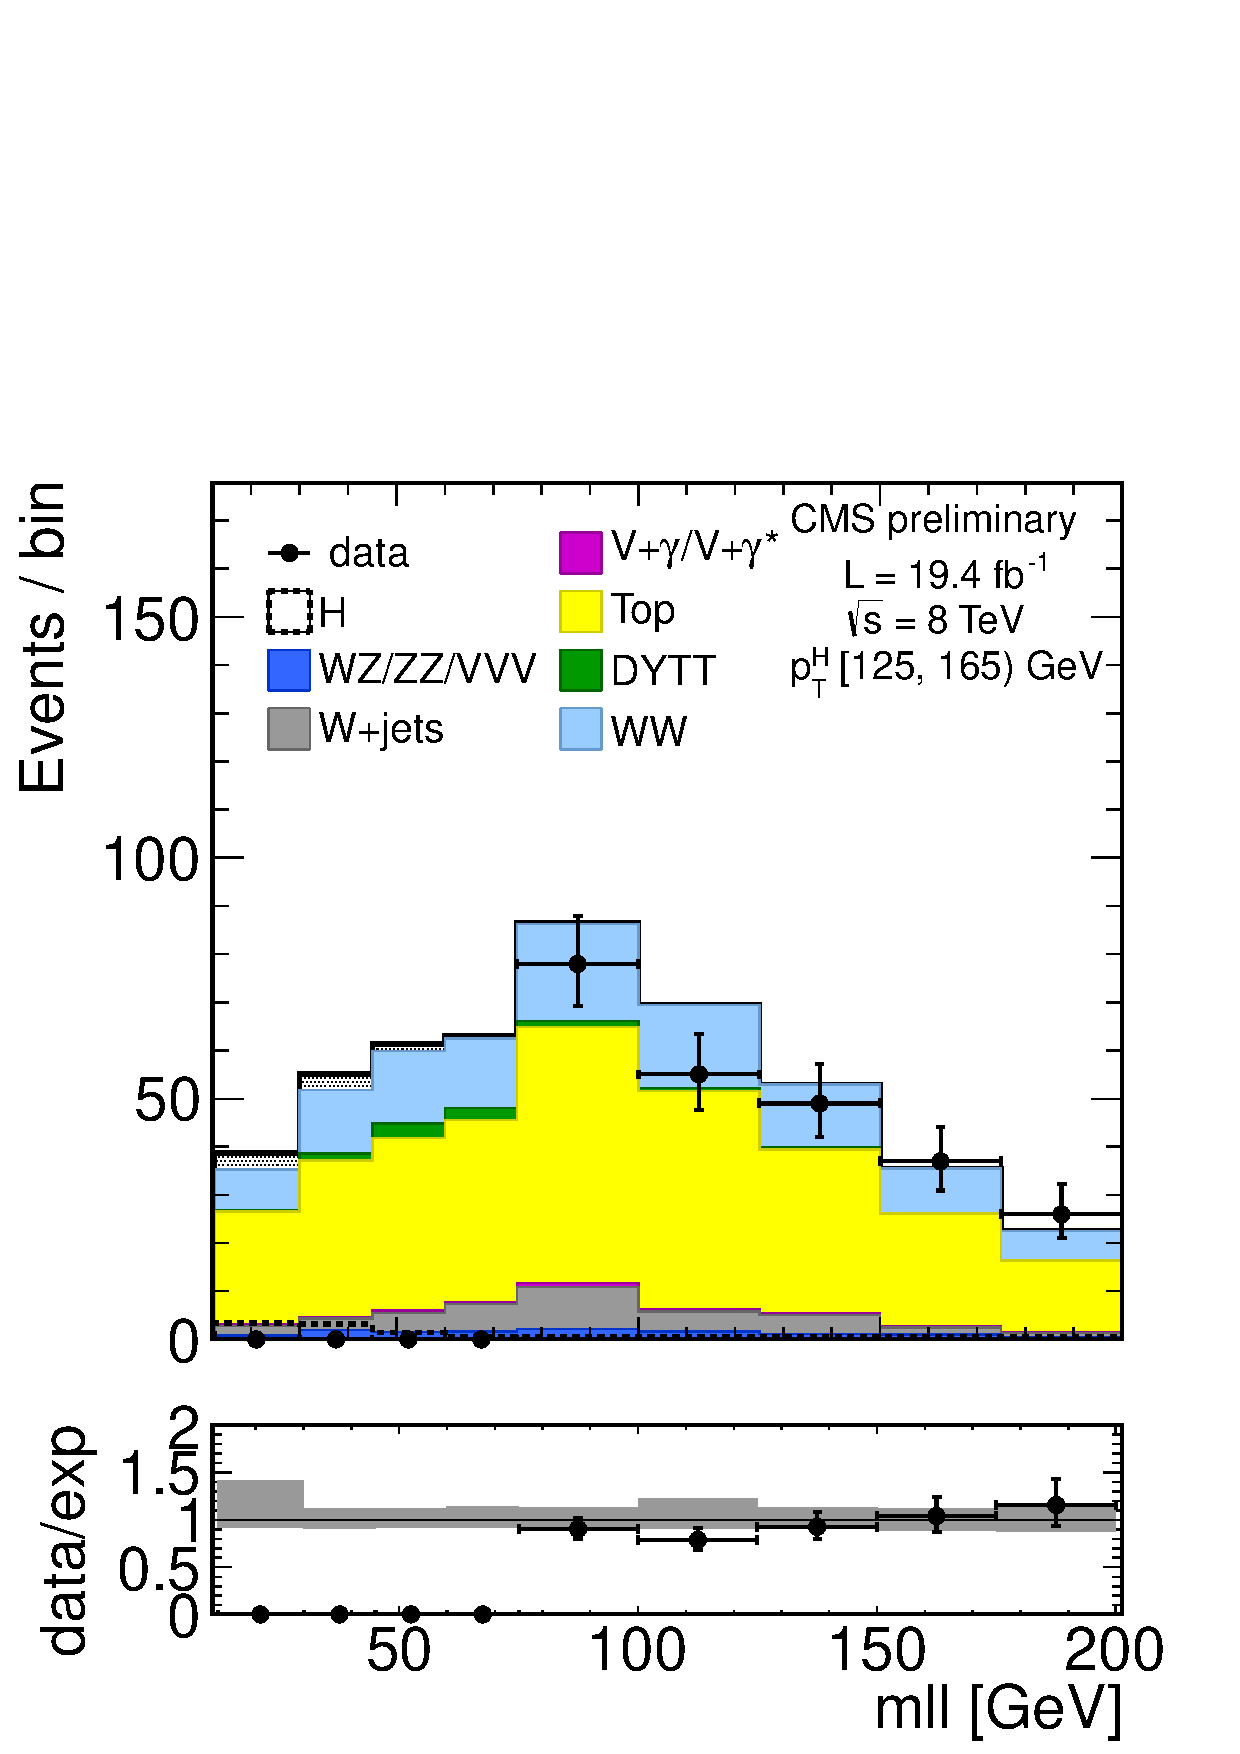
\includegraphics[width=0.35\textwidth]{images/mllBin4.pdf}
}
\subfigure[Bin6]{
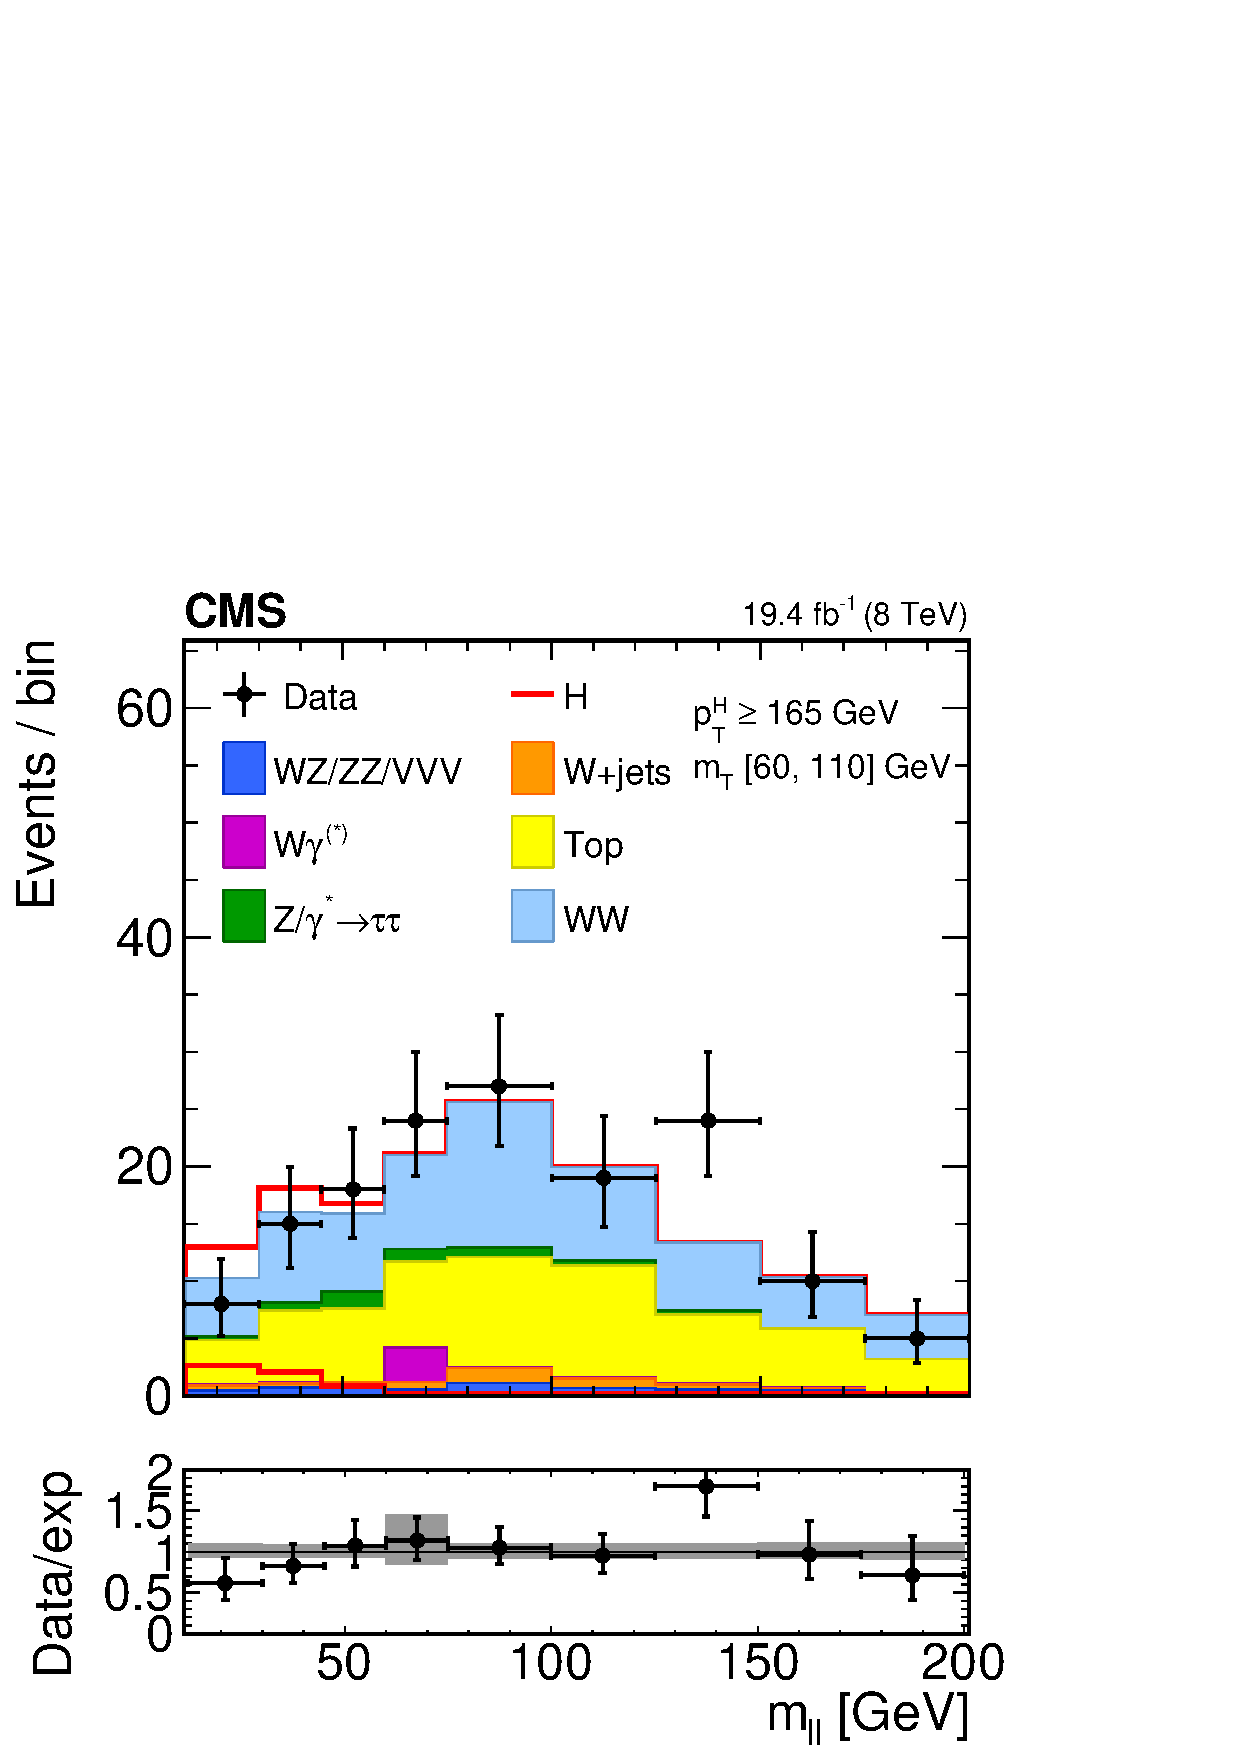
\includegraphics[width=0.35\textwidth]{images/mllBin5.pdf}
}
\caption{Control plots showing the \mll~distributions in every Higgs \pt bin. Data are superimposed in the region where the signal is expected to be negligible.}\label{fig:control_plots}

\end{figure}

As expected the Top background becomes more important while going to high values of \pth, accordingly to the higher jet multiplicity in that region. The discrepancy between MC prediction and data, especially for low values of Higgs \pt, is due WW background which in this plots is fixed to the MC cross section.

